\documentclass[a4paper]{article}
\usepackage{geometry}
\usepackage{graphicx}

\begin{document}

\section{Visual Studio Extension}
There already exists a Visual Studio Extension that allows support for the Dafny language within the Visual Studio IDE. By extending this, a programmer using this IDE can automatically analyse and remove any dead annotations without having to run a separate tool.\par
The analysis for dead annotations takes place after the editor has become idle for a period of time. The program text is resolved into a tree representation, which is sent to the Dary tool on a separate thread. Once this is complete, the thread will update and tag any spans of code in the editor that can be removed.\par

\begin{centering}
\vspace{0.5cm}
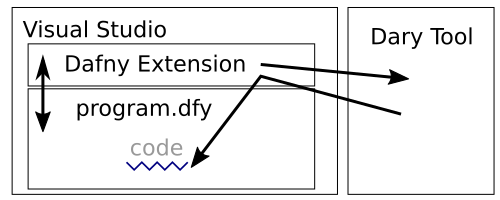
\includegraphics[scale=0.5]{drawing.png}\par
\textit{Basic overview of architecture}\par
\vspace{0.5cm}
\end{centering}

Using the Extensibility API provided by Visual Studio, we can then apply formatting and adornments use these tagged spans of code. In this case, the colour of dead code is reduced by making it less opaque, indicating that it is not really needed. An adornment, or \textit{squiggle}, is also added, to indicate that this is a warning that should be addressed.\par

\begin{centering}
\vspace{0.5cm}
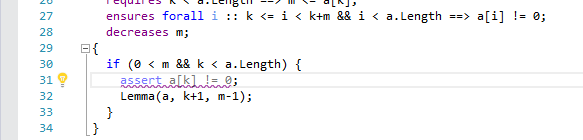
\includegraphics[scale=0.8]{tagLine2.png}\par
\textit{A lemma containing a dead assertion}\par
\vspace{0.5cm}
\end{centering}

Additionally, to make it simpler to remove these spans of code, the Visual Studio API for \textit{Quick Actions} is used. These offer an easy way to remove a single dead annotation, all of those in a function/method. These are accessed through either the usual quick actions menu or by right-clicking on tagged spans of code and using the Refactoring menu. Additionally, an item has been added to the main menu offered by the extension, under Dafny - Refactoring.\par

\begin{centering}
\vspace{0.5cm}
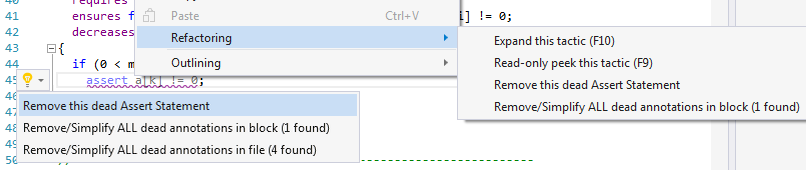
\includegraphics[scale=0.5]{qa_ctxt_3.png}\par
\textit{Quick actions and Context Menu}\par
\vspace{0.5cm}
\end{centering}

\end{document}